\fbox{%
    \fbox{%
        \parbox{\ifdefined\formurl0.85\else0.95\fi\textwidth}{%
            \begin{itemize}[\checkmark,nosep,leftmargin=16pt]
                \item No washroom breaks. Phones must be turned off. Using/carrying any notes during the exam is not allowed.
                      % \item At the end of the exam, both the \textbf{answer script} and the \textbf{question paper} must be returned to the invigilator.
                \item All \textbf{\numqinrange{\set}~question(s)} are compulsory. Marks allotted for each question are mentioned beside each question.
                      \ifthenelse{\equal{\numbonuspoints}{0}}{}{\item Bonus questions are indicated as ``\textbf{\textit{(bonus)}}" along with allotted marks.}
                \item Write your answers inside the indicated boxes (where applicable). If you run out of room, continue on the back page.
                \item Symbols have their usual meanings.
                      \ifdefined\deadline
                \item Last day of submission: \textbf{\deadline}.
                      \fi\ifdefined\formurl
                \item Submission link: \url{\formurl}
                      \fi
            \end{itemize}
        }%
    }%
}
\ifdefined\formurl
    \quad\qrcode{\formurl}
\fi

\ifdefstring{\insertomrsheet}{true}{
    \null\vspace{48pt}
    % 1pt = 1px
    \begin{tikzpicture}[scale=0.5, transform shape]
        \node[anchor=north west, inner sep=0] {
            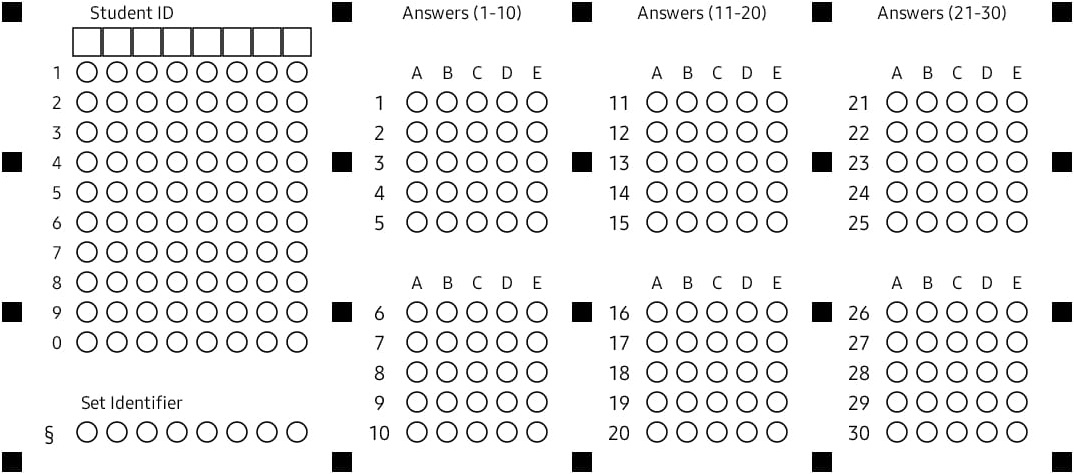
\includegraphics[width=1074pt, height=474pt]{omr.jpg}
        };
        \begin{scope}[x=1pt, y=1pt]
            \draw[fill=black]
            % using paint to find the center pixel
            % position of set identifier bubbles
            \foreach\ci in {1,...,8}{
                    \execifzero{\ci}{
                        (\inteval{87+(\ci-1)*30},-432) circle[radius=10]
                    }
                }
            ;
        \end{scope}
    \end{tikzpicture}
    \vspace{48pt}
}{
    \vspace{12pt}
}